\section{Games}

\project{Games!}{Computers and electronics are not just about having fun---you can play games as well!}

\subsection*{Equipment Required}

The circuit built in Section~\ref{s:buzzer}.

\begin{figure}[htbp]
  \centering
  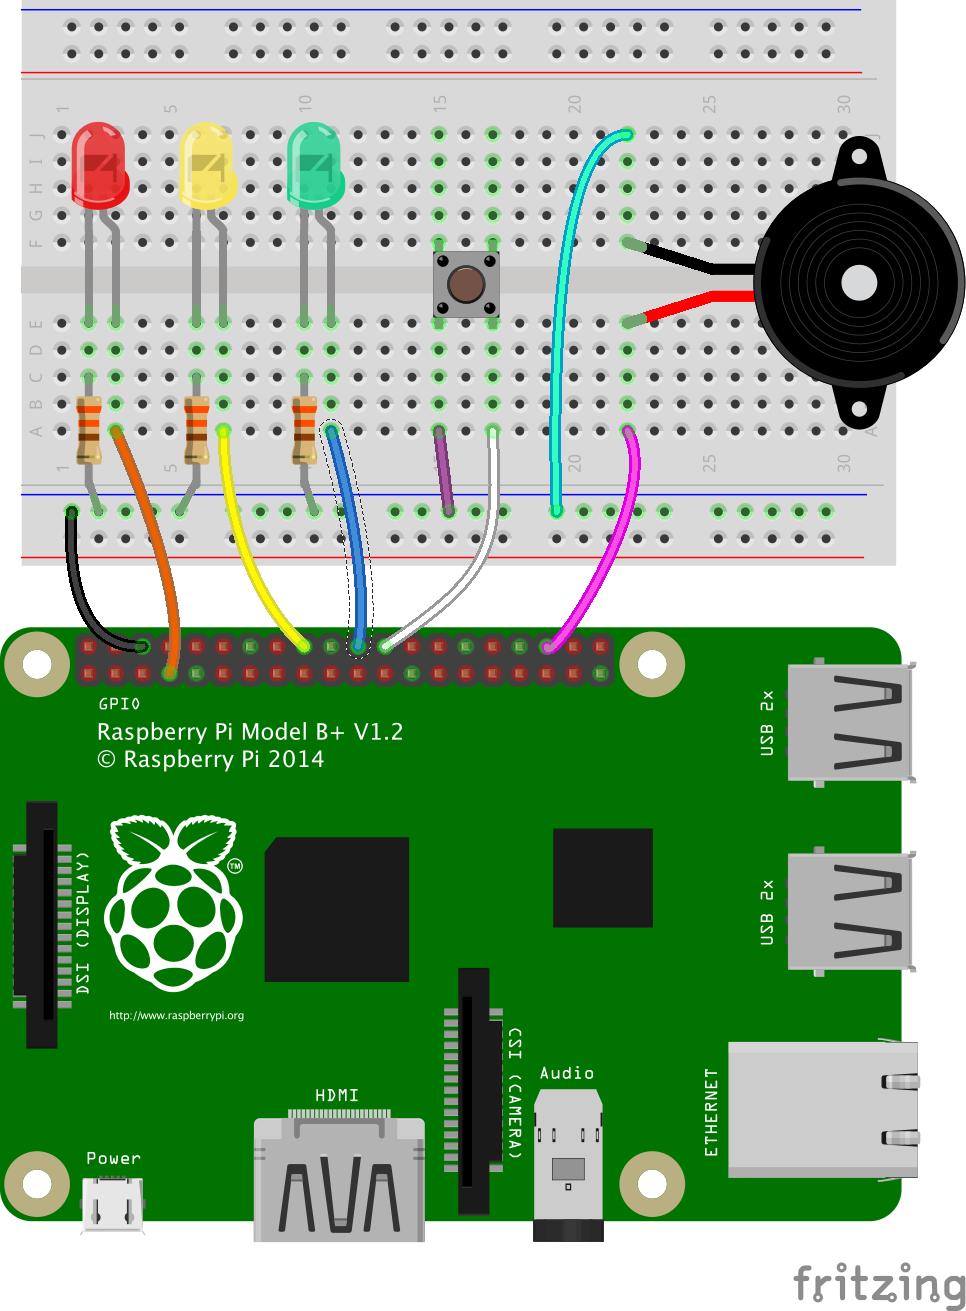
\includegraphics[width=0.75\textwidth]{buzzer-circuit}
\end{figure}

\subsection*{Exercises}

In this worksheet, you're not going to be given any code.  You are just going to be given some ideas for games you can make and play using the CamJam EduKit, and some hints that you might need.

\subsubsection*{Hints}

Random numbers can be generated with `RND(1)'.  This will generate a random number between 0 and 1.  To generate a number between 1 and X, you can use `INT(RND(1)*X+1)' as in the following code:
\begin{basic}
10 PRINT "RANDOM NUMBER BETEWEEN 1 AND 10: ";
20 PRINT INT(RND(1)*10+1)
\end{basic}

Print out instructions for the user to the screen using the `PRINT' command:
\begin{basic}
10 PRINT "TELL THE USER WHAT TO DO"
\end{basic}

\subsubsection*{Game 1---Reaction Timer}

Light the LEDs one at a time, going from Red to Green with one second in between.  After the green has been lit, wait a random length of time (say, between 1 and 5 seconds) before sounding the buzzer.  Time how long it takes from the buzzer sounding to the player pressing the button.

\subsubsection*{Game 2---Eat the Orange}

Randomly choose which LED to light.  Light it for 0.2 seconds.  If the player presses the button while the Amber LED is lit, they get a point.  Time how long it takes for them to get 10 points.

\subsubsection*{Game 3---Segment of Orange}

Change the colour of the LEDs from red, to amber, to green, to amber, and back to red every 0.1s.  If the player presses the button when the amber LED is lit, they get a point.  Only give them 10 chances to hit the button when the amber is lit.
